\documentclass[11pt]{article}
\pagestyle{empty}

\usepackage{amsfonts}
\usepackage{latexsym}
\usepackage{amssymb,amsthm,amsmath}
\usepackage{a4wide}
\usepackage[dvipsnames,usenames]{xcolor}
\usepackage{xcolor,colortbl}
\usepackage[all]{xy}
\usepackage{enumitem}
\usepackage{circuitikz}
\usepackage{tikz}
\usetikzlibrary{shapes.geometric}
\usetikzlibrary{arrows}
\usepackage[normalem]{ulem}
\usepackage{tikz}
\usetikzlibrary{automata,positioning}

\newcommand{\blank}{\setlength{\unitlength}{1pt}\begin{picture}(6,4.2)
\put(1,.5){\line(1,0){4}}
\multiput(1,.5)(4,0){2}{\line(0,1){2}}
\end{picture}
}

\newcommand{\nbullet}{\tc{NavyBlue}{--}\hspace*{1em}}
\newcommand{\rbullet}{\tc{OrangeRed}{--}\hspace*{1em}}


\begin{document}

\noindent {\large\sf Fundamentals of Computing}\qquad Autumn 
2013\hfill{\large\sf Coursework}

\bigskip
\begin{center}
\fbox{\parbox{14.3cm}{{\large\bf For return on 24 January 2014 \quad  (late submission: 7 February 2014)}}}
\end{center}

\mbox{} \hfill {\em Electronic submission: \underline{\bf pdf} files only}


%*****************************

\vspace{1.5cm} 
\noindent
%
1. {\bf (3\%)}  Construct the truth-table for the Boolean function given by the Boolean formula
%
$$
\neg \big(A \land (B \to C)\big) \land \neg B.
$$
%
Use the truth-table to realise this function by a formula with the  connectives $\neg,\ \lor,\ \land$ only. Simplify the formula in such a way that the corresponding Boolean circuit contains a minimal number of gates. Show the Boolean circuit.

\fbox{\parbox{\textwidth}{
%
$$
{\Large\textbf{Truth Table}}
$$
%

%
$$
\newcolumntype{a}{>{\columncolor{SpringGreen}}c}
 \begin{tabular}{ l*{2}{c} || l*{5}{c} | a | c}
         \textsl{$A$} & \textsl{$B$} & \textsl{$C$} & \textsl{$\neg$} & \textsl{$(A$} & \textsl{$\land$}& \textsl{($B$} & \textsl{$\to$} & \textsl{$C))$} & \textsl{$\land$} & \textsl{$\neg B$)} \\ \hline
         0 & 0 & 0 & 1 & & 0 & & 1 & & 1 & 1\\
         0 & 0 & 1 & 1 & & 0 & & 1 & & 1 & 1\\
         0 & 1 & 0 & 1 & & 0 & & 0 & & 0 & 0\\
         0 & 1 & 1 & 1 & & 0 & & 1 & & 0 & 0\\
         1 & 0 & 0 & 0 & & 1 & & 1 & & 0 & 1\\
         1 & 0 & 1 & 0 & & 1 & & 1 & & 0 & 1\\
         1 & 1 & 0 & 1 & & 0 & & 0 & & 0 & 0\\
         1 & 1 & 1 & 0 & & 1 & & 1 & & 0 & 0\\
\end{tabular}
$$
%
\\
%
$$
{\Large\textbf{Simplification}}
$$
%

\begin{enumerate}[itemsep=1em]
  \item{
    \textsl{$(\neg A \land \neg B \land \neg C ) \lor (\neg A \land \neg B \land C)$}
  }
  \item{
    \textsl{$(\neg(A \lor B) \land \neg C) \lor (\neg(A \lor B) \land C)$}
  }
  \item{
    \textsl{$\neg(A \lor B) \lor (\neg C \land C)$}
  }
  \item{
    \textsl{$\neg(A \lor B) \lor 0$}
  }
  \item{
    \textsl{$\neg(A \lor B)$}
  }
\end{enumerate}

%
$$
{\Large\textbf{Boolean Circuit}}
$$
%
\\
%
$$
\begin{circuitikz}
  \draw
    (0,0) node[or port] (myor) {}
    (1,0) node[not port] (mynot) {}
    
    (myor.in 1) node[left=0.5cm](a) {\textsl{$A$}} 
    (myor.in 2) node[left=0.5cm](b) {\textsl{$B$}} 
    
    (a) -- (myor.in 1)
    (b) -- (myor.in 2)
    (myor.out) -- (mynot.in)
  ;
\end{circuitikz}
$$
%
}}



%**************************

\bigskip
\noindent
%
2. {\bf (3\%)} Are the following Boolean formulas equivalent? Explain your answer.
%
\begin{enumerate}
\item[(a)] $A \to ( B \land C)$ and $(A\to B) \land (A \to C)$
\\

\fbox{\parbox{\textwidth}{
%
$$
\newcolumntype{a}{>{\columncolor{SpringGreen}}c}
 \begin{tabular}{ l*{2}{c} || c | a | l*{3}{c}}
        \textsl{$A$} & \textsl{$B$} & \textsl{$C$} & \textsl{$A$} & \textsl{$\to$} & \textsl{$(B$}& \textsl{$\land$} & \textsl{$C)$} \\ \hline
        0 & 0 & 0 &  & 1 &  & 0 & \\
        0 & 0 & 1 &  & 1 &  & 0 & \\
        0 & 1 & 0 &  & 1 &  & 0 & \\
        0 & 1 & 1 &  & 1 &  & 1 & \\
        1 & 0 & 0 &  & 0 &  & 0& \\
        1 & 0 & 1 &  & 0 &  & 0 & \\
        1 & 1 & 0 &  & 0 &  & 0 & \\
        1 & 1 & 1 &  & 1 &  & 1 & \\
 \end{tabular}
 $$
%
\\
 %
$$
 \newcolumntype{a}{>{\columncolor{SpringGreen}}c}
 \begin{tabular}{ l*{2}{c} || l*{2}{c} |a| l*{2}{c}}
        \textsl{$A$} & \textsl{$B$} & \textsl{$C$} & \textsl{$(A$} & \textsl{$\to$} & \textsl{$B)$} & \textsl{$\land$} & \textsl{$(A$} & \textsl{$\to$} & \textsl{$C)$}\\ \hline
        0 & 0 & 0 &  & 1 &  & 1 &  & 1 \\
        0 & 0 & 1 &  & 1 &  & 1 &  & 1 \\
        0 & 1 & 0 &  & 1 &  & 1 &  & 1 \\
        0 & 1 & 1 &  & 1 &  & 1 &  & 1 \\
        1 & 0 & 0 &  & 0 &  & 0 &  & 0 \\
        1 & 0 & 1 &  & 0 &  & 0 &  & 1 \\
        1 & 1 & 0 &  & 1 &  & 0 &  & 0 \\
        1 & 1 & 1 &  & 1 &  & 1 &  & 1 \\
 \end{tabular}
$$
%
}}
\\
%
$$
{\large\textbf{Yes they are equivalent}}
$$
%
\newpage

\item[(b)] $(A \land B) \to C$ and $(\neg C\to \neg A) \land (\neg C \to \neg B)$ \\

\fbox{\parbox{\textwidth}{
%
$$
\newcolumntype{a}{>{\columncolor{SpringGreen}}c}
 \begin{tabular}{ l*{2}{c} || l*{2}{c} |a| c}
        \textsl{$A$} & \textsl{$B$} & \textsl{$C$} & \textsl{$(A$} & \textsl{$\land$} & \textsl{$B)$} & \textsl{$\to$} & \textsl{$C$}\\ \hline
        0 & 0 & 0 &  & 0 &  & 1 &  \\
        0 & 0 & 1 &  & 0 &  & 1 &  \\
        0 & 1 & 0 &  & 0 &  & 1 &  \\
        0 & 1 & 1 &  & 0 &  & 1 &  \\
        1 & 0 & 0 &  & 0 &  & 1 &  \\
        1 & 0 & 1 &  & 0 &  & 1 &  \\
        1 & 1 & 0 &  & 1 &  & 0 &  \\
        1 & 1 & 1 &  & 1 &  & 1 &  \\
 \end{tabular}
$$
% 
%
$$
 \newcolumntype{a}{>{\columncolor{SpringGreen}}c}
 \begin{tabular}{ l*{2}{c} || c l c | a | c l c}
       \textsl{$A$} & \textsl{$B$} & \textsl{$C$} & \textsl{$(\neg C$} & \textsl{$\to$} & \textsl{$\neg A)$} & \textsl{$\land$} & \textsl{$(\neg C$} & \textsl{$\to$} & \textsl{$\neg B)$}\\ \hline
        0 & 0 & 0 & 1 & 1 & 1 & 1 & 1 & 1 & 1\\
        0 & 0 & 1 & 0 & 1 & 1 & 1 & 0 & 1 & 1\\
        0 & 1 & 0 & 1 & 1 & 1 & 0 & 1 & 0 & 0\\
        0 & 1 & 1 & 0 & 1 & 1 & 1 & 0 & 1 & 0 \\
        1 & 0 & 0 & 1 & 0 & 0 & 0 & 1 & 1 & 1 \\
        1 & 0 & 1 & 0 & 1 & 0 & 1 & 0 & 1 & 1 \\
        1 & 1 & 0 & 1 & 0 & 0 & 0 & 1 & 0 & 0 \\
        1 & 1 & 1 & 0 & 1 & 0 & 1 & 0 & 1 & 0 \\
 \end{tabular}
$$
%
}}
\\
%
$$
{\large\textbf{No they are not equivalent}}
$$
%

\item[(c)] $(A \lor B) \to C$ and $(A\to B) \lor (A \to C)$
\\
\fbox{\parbox{\textwidth}{
%
$$
\newcolumntype{a}{>{\columncolor{SpringGreen}}c}
 \begin{tabular}{ l*{2}{c} ||  l*{2}{c} |a| c}
        \textsl{$A$} & \textsl{$B$} & \textsl{$C$} & \textsl{$(A$} & \textsl{$\lor$} & \textsl{$B)$} & \textsl{$\to$} & \textsl{$C$}\\ \hline
        0 & 0 & 0 &  & 0 &  & 1 &   \\
        0 & 0 & 1 &  & 0 &  & 1 &   \\
        0 & 1 & 0 &  & 1 &  & 0 &   \\
        0 & 1 & 1 &  & 1 &  & 1 &   \\
        1 & 0 & 0 &  & 1 &  & 0 &   \\
        1 & 0 & 1 &  & 1 &  & 1 &   \\
        1 & 1 & 0 &  & 1 &  & 0 &   \\
        1 & 1 & 1 &  & 1 &  & 1 &   \\
 \end{tabular}
 $$
%

%
$$
 \newcolumntype{a}{>{\columncolor{SpringGreen}}c}
 \begin{tabular}{ l*{2}{c} || c l c | a | c l c}
        \textsl{$A$} & \textsl{$B$} & \textsl{$C$} & \textsl{$(A$} & \textsl{$\to$} & \textsl{$B)$} & \textsl{$\lor$} & \textsl{$(A$} & \textsl{$\to$} & \textsl{$C)$}\\ \hline
        0 & 0 & 0 &  & 1 &  & 1 & & 1\\
        0 & 0 & 1 &  & 1 &  & 1 & & 1\\
        0 & 1 & 0 &  & 1 &  & 1 & & 1\\
        0 & 1 & 1 &  & 1 &  & 1 & & 1\\
        1 & 0 & 0 &  & 0 &  & 0 & & 0\\
        1 & 0 & 1 &  & 0 &  & 1 & & 1\\
        1 & 1 & 0 &  & 1 &  & 1 & & 0\\
        1 & 1 & 1 &  & 1 &  & 1 & & 1\\
 \end{tabular}
 $$
%
}}
\\
%
$$
{\large\textbf{No they are not equivalent}}
$$
%
\\
\end{enumerate}


%*******************

\bigskip
\noindent
%
3. {\bf (3\%)} A parity function is a Boolean function whose value is 1 if the input has an odd number of ones. Design a Boolean circuit for the 2-bit parity function. Show your working. (Hint: you may find  XOR gates useful.)

\fbox{\parbox{\textwidth}{
%
$$
\begin{tabular}{c c || c}
  \textsl{$A$} & \textsl{$B$}\\ \hline
  0 & 0 & 0 \\
  0 & 1 & 1 \\
  1 & 0 & 1 \\
  1 & 1 & 0 \\
\end{tabular}
$$
%
\\
%
$$
\begin{circuitikz}
  \draw
    (0,0) node[xor port] (myor) {}
    
    (myor.in 1) node[left=0.5cm](a) {\textsl{$A$}} 
    (myor.in 2) node[left=0.5cm](b) {\textsl{$B$}} 
    
    (a) -- (myor.in 1)
    (b) -- (myor.in 2)
  ;
\end{circuitikz}
$$
%
}}

%********************

\bigskip
\noindent
%
4. {\bf (3\%)} Suppose $\alpha = a_{31} a_{30} \dots a_1 a_0$ is a 32-bit binary word. Consider the 32-bit binary 
word $\beta = b_{31} b_{30} \dots b_1 b_0$ computed by the following algorithm: scan $\alpha$ from right 
to left and copy its bits to $\beta$ until the first 1 is found (which is also copied to $\beta$); after that, 
copy the Boolean negations of the bits in $\alpha$. For example, $\alpha = 10100\dots 00$ is transformed to $\beta = 01100\dots 00$. Explain what this algorithm computes if $\alpha$ and $\beta$ are interpreted as binary numbers.
\linebreak
\linebreak
\fbox{\parbox{\textwidth}{
	Given a two's compliment binary number, the algorithm computes the conversion into a binary number.
}}
\\
%******************
\newpage
\bigskip
\noindent
%
5. {\bf (6\%)} Given the machine 32-bit word
%
$$
1100 \ 0001\ 0011 \ 0000 \ 0000 \ 0000\ 0000 \ 0000
$$
%
find the decimal number represented by this word assuming that it is
%
\begin{itemize}
\item[(a)] a two's complement integer;
  \begin{itemize}
    \item[] {
       \fbox{\parbox{\textwidth}{
         \begin{enumerate}
           \item {
             Read the first character from the left of the word to get the sign of the integer it represents. In this case it is a one so the number is negative.
           }
           \item{
             Use the two's compliment algorithm to convert it into a binary number. Starting from the right of the word, move to the first one :
              \begin{itemize}
               \item{
                 1100 0001 001\uline{1} 00...00
               }
             \end{itemize}
           }
           \item{
           Move left, from the first on flipping the bit after the first one until you reach the far left:
            \begin{itemize}
               \item{
                   1100 0001 00\uline{0}1 00...00
               }
                \item{
                   1100 0001 0\uline{1}01 00...00
               }
                \item{
                   1100 0001 \uline{1}101 00...00
               }
                \item{
                   1100 000\uline{0} 1101 00...00
               }
               \item{
                   1100 00\uline{1}0 1101 00...00
               }
               \item{
                   1100 0\uline{1}10 1101 00...00
               }
               \item{
                   1100 \uline{1}110 1101 00...00
               }
               \item{
                   110\uline{1} 1110 1101 00...00
               }
               \item{
                   11\uline{1}1 1110 1101 00...00
               }
               \item{
                   1\uline{0}11 1110 1101 00...00
               }
               \item{
                   \uline{0}011 1110 1101 00...00
               }
             \end{itemize}
           }
           \item{
           	Then add all the base two 1's together to get the integer:
	         \begin{itemize}
	           \item{$2^{29}$ + $2^{28}$ + $2^{27}$ + $2^{26}$ + $2^{25}$ + $2^{23}$ + $2^{22}$ + $2^{20}$ = 1053818880}
	         \end{itemize}
           }
           \item{
           	And multiply it by the sign, which is -1:
	        \begin{itemize}
	           \item{-1(1053818880) = -1053818880}
	         \end{itemize}
           }
         \end{enumerate}
       }}
    }
  \end{itemize}

\item[(b)] an unsigned integer;
 \begin{itemize}
    \item[] {
       \fbox{\parbox{\textwidth}{
         As an unsigned integer, add the base two ones together:\\
         $2^{31}$ + $2^{30}$ + $2^{24}$ + $2^{21}$ + $2^{20}$ = 3241148416
       }}
    }
 \end{itemize}
\newpage
\item[(c)] a single precision IEEE 754 floating-point number.
 \begin{itemize}
    \item[] {
       \fbox{\parbox{\textwidth}{
         \textsl{$(-1)^S$ $\times$ (1 + F) $\times$ $2^E$}\\
         S = Sign \\
         F = fraction  (0 \textless \ F \textless 1)\\
         E = Exponent - Bias\\
         Bias = 127 for single precision\\ 
         
         If the first character of the word is a one then the sign is negative: \\
         S = 1\\ 
         
         The next eight bits make up the exponent: \\
         E = 100 0001 0 = $2^7$ + $2^1$ = 128 + 2 = 130 - Bias = 130 - 127 = 3\\
         \\
         F = 011 \ 0000 \ 0000 \ 0000\ 0000 \ 0000\\
         Going from left to right, with left as the zero point and going into the negative:\\
         $2^{-2}$ + $2^{-3}$ = 0.25 + 0.125 = 0.375\\
         \\
         \textsl{$(-1)^1$ $\times$ (1 + 0.375) $\times$ $2^3$}\\
          \textsl{$-1$ $\times$ 1.375 $\times$ $8$}\\
          The answer is -11
       }}
    }
 \end{itemize}
\end{itemize}


%********************


\bigskip
\noindent
%
6. {\bf (6\%)} Find computer representations of the following numbers:
%
\begin{enumerate}
\item[(a)] $-1022$ as a two's complement 32-bit binary number;

\begin{itemize}
    \item[] {
       \fbox{\parbox{\textwidth}{
         First turn it into a positive binary number:\\
          S = -1\\
          N = 1022
           \begin{itemize}
             \item[]{
                1022/2 = 511 $\to$ 0
             }
             \item[]{
             	511/2 = 255.5 $\to$ 1 
             }
             \item[]{
             	255/2 = 127.5 $\to$ 1
             }
             \item[]{
             	127/2 = 63.5 $\to$ 1
             }
             \item[]{
             	63/2 = 31.5 $\to$ 1
             }
             \item[]{
             	31/2 = 15.5 $\to$ 1
             }
             \item[]{
             	15/2 = 7.5 $\to$ 1
             }
             \item[]{
             	7/2 = 3.5 $\to$ 1
             }
             \item[]{
             	3/2 = 1.5 $\to$ 1
             }
             \item[]{
             	1/2 = 0.5 $\to$ 1
             }
           \end{itemize}
           Now we have 0...0011\ 1111\ 1110\\
           Since it needs to be a two's compliment number we need to use the algorithm from before to flip the bits.\\
           Which becomes: 1...1100\ 0000\ 0010
           Since it is a negative number we leave the first character as a one:\\ \\
           Answer = 1111\ 1111\ 1111\ 1111\ 1111\ 1100\ 0000\ 0010
       }}
    }
\end{itemize}

\item[(b)] $-32.75$ as an IEEE 754 32-bit floating-point number;

\begin{itemize}
    \item[] {
       \fbox{\parbox{\textwidth}{
       		 
        		\begin{tabular}{|c|c|c|} 
		\hline
		S & E (Exponent) & F (Fraction) \\ 
		\hline
		1bit & 8 bits & 23 bits \\
		\hline
		\end{tabular}\\ \\
		Bias = 127 \\
		S = 1 since it is a negative number. \\
		\\
		32.75\\
		32 = 10000 in binary\\
		0.75 $\times$ 2 = 1.5 $\to$ 1 \\
		0.5 $\times$ 2 = 1 $\to$ 1 \\
		1.1 \\
		\\
		100001.1 \\ \\
		1.000011 $\times$ $2^5$ = 100001.1 \\
		E = 5 + 127 = 132 = 10000100 \\
		F = 000011 \\ \\
		\begin{tabular}{|c|c|c|} 
		\hline
		1 & 100 0010 0 & 000 0110 0000 0000 0000 0000 \\
		\hline
		S & E (Exponent) & F (Fraction) \\ 
		\hline
		\end{tabular}
       }}
    }
\end{itemize}

\item[(c)] $77$ as a two's complement 32-bit binary number.

\begin{itemize}
    \item[] {
       \fbox{\parbox{\textwidth}{
 	  \begin{itemize}
             \item[]{
             	77/2 = 38.5 $\to$ 1
             }
             \item[]{
             	38/2 = 19 $\to$ 0
             }
             \item[]{
             	19/2 = 9.5 $\to$ 1
             }
             \item[]{
             	9/2 = 4.5 $\to$  1
             }
             \item[]{
             	4/2 = 2 $\to$ 0
             }
             \item[]{
             	2/2 = 1 $\to$ 0
             }
             \item[]{
             	1/2 = 0.5 $\to$ 1
             }
          \end{itemize}       
          Answer = 0000\ 0000\ 0000\ 0000\ 0000\ 0000\ 0100\ 1101
       }}
    }
\end{itemize}

\end{enumerate}


%********************

\bigskip
\noindent
%
7. {\bf (6\%)}  Consider the following finite automaton:
\[
\xymatrix @C+12mm {
{\txt{$>$}}\!\!\!\!\!\!\!\!\!\!\!\!\!\!\!\!\!\!\!\!\!\!\!\!\!\!\!\!\!\!
\!\!\!\!\!\!\!\!\!\!\!\!\!\!\!\!\!\!\!\!\!\!\!\!\!\!\!\!\!\!\!\!\!\!
&*++[o][F=]{s} \ar@(ul,ur)^b  \ar@<.5ex>[r]^\varepsilon
&*++[o][F-]{p} \ar@(ul,ur)^a  \ar@<.5ex>[l]^a
& \
}
\]
%
\begin{itemize}
\item[(a)]
Give all the computations of the automaton on the input strings 
$aab$, $aba$, and $\varepsilon$, 
and determine if the strings are accepted.
\begin{itemize}
    \item[] {
       \fbox{\parbox{\textwidth}{
 	  \begin{itemize}
	    
             \item[]{
             Input: $aab$\\
             Computation: 
             	\begin{itemize}
			\item{
				(s, aab), (p, aab), (p, ab), (s, b), (s, $\varepsilon$) Accepted
			}
			\item{
				(s, aab), (p, aab), (s, ab), (p, ab), (s, b), (s, $\varepsilon$) Accepted
			}
			\item{
				(s, aab), (p, aab), (p, ab), (p, b) stuck
			}
			\item{
				(s, aab), (p, aab), (p, ab), (s, b), (p, b) stuck
			}
			\item{
				(s, aab), (p, aab), (s, ab),  (p, ab),  (s, b), (s, $\varepsilon$) Accepted \\
			}
		\end{itemize}
		word $aab$ is Accepted.\\
             }
             
             \item[]{
             Input: $aba$\\
             Computation: 
             	\begin{itemize}
			\item{
				(s, aba), (p, aba), (p, ba) stuck
			}
			\item{
				(s, aba), (p, aba), (s, ba), (s, a), (p, a), (p, $\varepsilon$) stuck
			}
			\item{
				(s, aba), (p, aba), (s, ba), (s, a), (p, a), (s, $\varepsilon$) Accepted
			}
			\item{
				(s, aba), (p, aba), (s, ba), (p, ba) stuck \\ 
			}
		\end{itemize}
		word $aba$ is Accepted.\\
             }
             
             \item[]{
             Input: $\varepsilon$\\
             Computation: 
             	\begin{itemize}
			\item{
				(s, $\varepsilon$), (p, $\varepsilon$) stuck
			}
			\item{
				(s, $\varepsilon$) Accepted\\
			}			
		\end{itemize}
		word  $\varepsilon$ is Accepted.\\
             }           
          \end{itemize}
      }}
   }
\end{itemize}

\item[(b)]
Describe the language accepted by the automaton in English.
\begin{itemize}
    \item[] {
       \fbox{\parbox{\textwidth}{
 	  \begin{itemize}
             \item[]{
             	The language accepts any amount of a's and b's and the empty word.
             }
          \end{itemize}
      }}
   }
\end{itemize}

\item[(c)]
Describe the language accepted by the automaton by means of a
regular expression.
\begin{itemize}
    \item[] {
       \fbox{\parbox{\textwidth}{
 	  \begin{itemize}
             \item[]{
             	(a $\cup$ b)*
             }
          \end{itemize}
      }}
   }
\end{itemize}

\item[(d)]
Describe the language accepted by the automaton by means of a context-free grammar.
\end{itemize}
\begin{itemize}
    \item[] {
       \fbox{\parbox{\textwidth}{
 	  \begin{itemize}
             \item[]{
             	S $\to$ $\varepsilon$ \\
		S $\to$ aS \\
		S $\to$ bS 
             }
          \end{itemize}
      }}
   }
\end{itemize}

%*******************
\newpage
\medskip
\noindent
%
8. {\bf (10\%)} 
Transform, using the subset construction, 
the following nondeterministic finite automaton into an
equivalent deterministic finite automaton.  Show your working.
%
\[
\UseTips
\xymatrix {
{\txt{$>$}}\!\!\!\!\!\!\!\!\!\!\!\!\!\!\!\!\!\!\!\!\!\!\!\!\!\!\!
&*++[o][F-]{s} \ar@(ul,ur)^a \ar@<.5ex>[r]^a \ar@/_2pc/[rr]_\varepsilon 
&*++[o][F=]{r} \ar@(ul,ur)^a \ar@<.5ex>[r]^b \ar@<.5ex>[l]^{b} 
&*++[o][F=]{t} \ar@(ul,ur)^b \ar@<.5ex>[l]^{a} 
& \
}
\]
\begin{itemize}
    \item[] {
       \fbox{\parbox{\textwidth}{
%
$$
\begin{tabular}{c || c c}
  & \textsl{$A$} & \textsl{$B$}\\ \hline
  s & {s,t} & $\varepsilon$ \\
  t & t & {s,r} \\
  r & t & r \\
  {s,t} & {s,t} & {s,r} \\
  {s,r} & {s,t} & r \\
  {t,r} & t & {s,r} \\
  {s,t,r} & {s,t} & {s,r} \\
  $\varepsilon$ & $\varepsilon$ & $\varepsilon$
\end{tabular}
$$
%
\begin{center}
  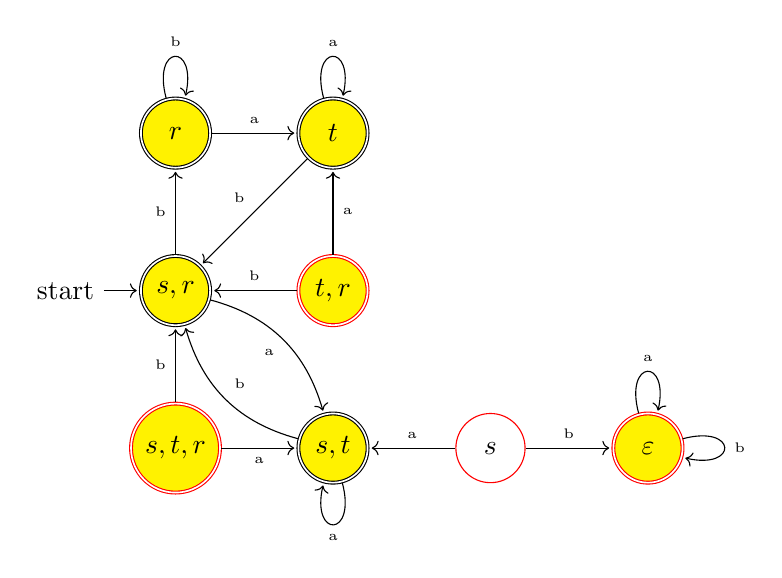
\begin{tikzpicture}[shorten >=1pt,node distance=2cm,on grid,auto] [!h]
      
      \node[state,accepting, fill=yellow] (r) {$r$};   
      \node[state,accepting, fill=yellow] (t) [right=of r] {$t$};
      \node[state, initial,accepting, fill=yellow] (a) [below=of r] {$s,r$};       
      \node[state,accepting, fill=yellow, draw=red] (c) [right=of a] {$t,r$};
      \node[state,accepting, fill=yellow, draw=red] (d) [below=of a] {$s,t,r$}; 
      \node[state,accepting, fill=yellow] (b) [right=of d] {$s,t$};   
      \node[state](s) [right=of b, draw=red](s) {$\textsl{$s$}$};
      \node[state, accepting, fill=yellow, draw=red] (e) [right=of s]  {$\textsl{$\varepsilon$}$};

       \path[->] 
          (s) edge node {\tiny b} (e)       
          (e) edge [loop above] node {\tiny a} (e)
          (e) edge [loop right] node {\tiny b} (e)
          (s) edge node [swap] {\tiny a} (b)
          (b) edge [bend left, swap] node {\tiny b} (a)
          (a) edge [bend left, swap] node {\tiny a} (b)
          (a) edge node {\tiny b} (r)
          (b) edge [loop below] node {\tiny a} (b)
          (c) edge node [swap] {\tiny b} (a)
          (c) edge node [swap] {\tiny a} (t)
          (t) edge node [swap] {\tiny b} (a)
          (t) edge [loop above] node {\tiny a} (t)
          (r) edge node {\tiny a} (t)
          (r) edge [loop above] node {\tiny b} (r)
          (d) edge node [swap] {\tiny a} (b)
          (d) edge node {\tiny b} (a)          
      ;
  \end{tikzpicture}
\end{center}

\begin{center}
  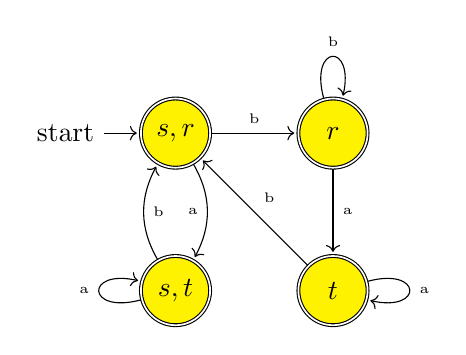
\begin{tikzpicture}[shorten >=1pt,node distance=2cm,on grid,auto] [!h]
	\node[state, initial,accepting, fill=yellow] (a) {$s,r$}; 
	 \node[state,accepting, fill=yellow] (b) [below=of a] {$s,t$}; 
	 \node[state,accepting, fill=yellow] (r) [right=of a] {$r$}; 
	 \node[state,accepting, fill=yellow] (t) [right=of b] {$t$};
	 
	  \path[->] 
	    (b) edge [bend left, swap] node {\tiny b} (a)
            (a) edge [bend left, swap] node {\tiny a} (b)
            (t) edge [loop right] node {\tiny a} (t)
            (t) edge node [swap] {\tiny b} (a)
            (r) edge [loop above] node {\tiny b} (r)
            (r) edge node {\tiny a} (t)
            (a) edge node {\tiny b} (r)
            (b) edge [loop left] node {\tiny a} (b)
	  ;
  \end{tikzpicture}
\end{center}
    }}
   }
\end{itemize}
What is the language of this automaton.
\begin{itemize}
    \item[] {
      \fbox{
        \parbox{\textwidth}{\centering
      		This language accepts any number of a's and b's.
        }
     }
  }
\end{itemize}

%***********************


\bigskip
\noindent
%
9. {\bf (7\%)}
Design a (deterministic or nondeterministic) finite
automaton $A$ such that $L(A)$ consists of all strings over the alphabet
$\{0,1\}$ that begin with $01$ and do not end with $11$. Find a regular expression representing the language $L(A)$.

\begin{itemize}
    \item[] {
      \fbox{
        \parbox{\textwidth}{
          \begin{center}
	   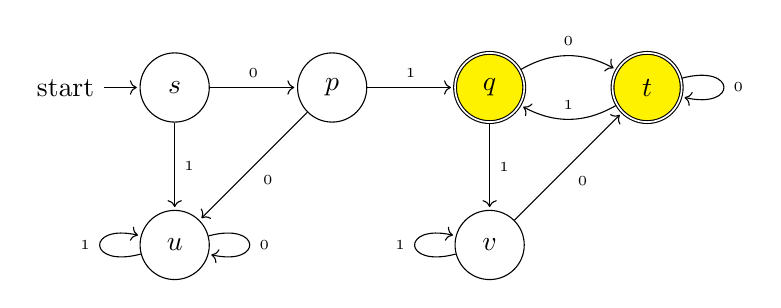
\begin{tikzpicture}[shorten >=1pt,node distance=2cm,on grid,auto] [!h]
	     \node[state, initial] (s) {$s$};
	     \node[state] (p) [right=of s] {$p$};
	     \node[state] (u) [below=of s] {$u$};
	     \node[state, accepting, fill=yellow] (q) [right=of p] {$q$};
	     \node[state, accepting, fill=yellow] (t) [right=of q] {$t$};
	     \node[state] (v) [below=of q] {$v$};
				
	     \path[->]
	     	(s) edge node {\tiny 0} (p)
		(s) edge node {\tiny 1} (u)
		(u) edge [loop left] node {\tiny 1} (u)
		(u) edge [loop right] node {\tiny 0} (u)
		(p) edge node {\tiny 0} (u)
		(p) edge node {\tiny 1} (q)
		(q) edge node {\tiny 1} (v)
		(q) edge [bend left] node {\tiny 0} (t)
		(t) edge [bend left, swap] node {\tiny 1} (q)
		(t) edge [loop right] node {\tiny 0} (t)
		(v) edge [swap] node {\tiny 0} (t)
		(v) edge [loop left] node {\tiny 1} (v)
	      ;
	   \end{tikzpicture}
         \end{center}
        }
     }
  }
\end{itemize}

\begin{itemize}
    \item[] {
      \fbox{
        \parbox{\textwidth}{\centering
		01((0 $\cup$ 1)*(0 $\cup$ 01))*        
        }
     }
  }
\end{itemize}

%******************

\medskip
\noindent
%
10. {\bf (6\%)} Design a (deterministic or nondeterministic) finite automaton $A$ such that $L(A)$ consists of all strings over the alphabet $\{0,1\}$ whose third symbol from the right end is $1$ (for example, 100101 is in $L(A)$, but 100011 is not). 
Find a regular expression representing $L(A)$. 
\begin{itemize}
    \item[] {
      \fbox{
        \parbox{\textwidth}{
          \begin{center}
	   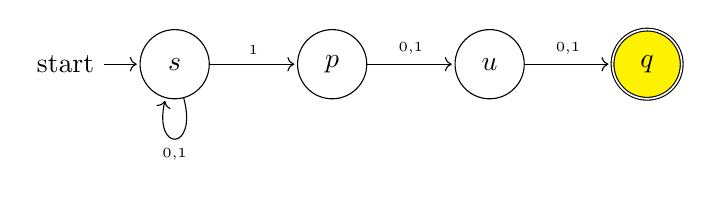
\begin{tikzpicture}[shorten >=1pt,node distance=2cm,on grid,auto] [!h]
	     \node[state, initial] (s) {$s$};
	     \node[state] (p) [right=of s] {$p$};
	     \node[state] (u) [right=of p] {$u$};
	     \node[state, accepting, fill=yellow] (q) [right=of u] {$q$};

	     \path[->]
	       (s) edge node {\tiny {1}} (p)
	       (s) edge [loop below] node {\tiny {0,1}} (p)
	       (p) edge node {\tiny {0,1}} (u)
	       (u) edge node {\tiny {0,1}} (q)
	     ;
            \end{tikzpicture}
          \end{center}
        }
     }
  }
\end{itemize}

\begin{itemize}
    \item[] {
      \fbox{
        \parbox{\textwidth}{\centering
		(0 $\cup$ 1)*1(0 $\cup$ 1)(0 $\cup$ 1)
        }
     }
  }
\end{itemize}
%**********************

\medskip
\noindent
%
11. {\bf (8\%)} Convert the regular language 
$L\bigl[\,x\bigl((y\cup x)^\ast x\bigr)^\ast y\,\bigr]$
to a finite automaton accepting it.
\begin{itemize}
    \item[] {
      \fbox{
        \parbox{\textwidth}{
          \begin{center}
	   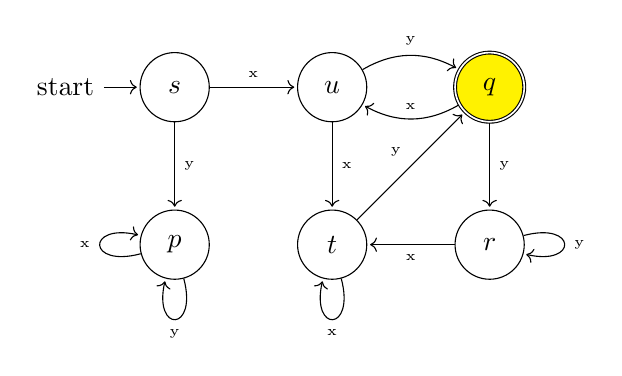
\begin{tikzpicture}[shorten >=1pt,node distance=2cm,on grid,auto] [!h]
	     \node[state, initial] (s) {$s$};
	     \node[state] (p) [below=of s] {$p$};
	     \node[state] (u) [right=of s] {$u$};
	     \node[state, accepting, fill=yellow] (q) [right=of u] {$q$};
	     \node[state] (t) [below=of u] {$t$};
	     \node[state] (r) [right=of t] {$r$};
	     
	     \path[->]
  	       (s) edge node {\tiny y} (p)
	       (s) edge node {\tiny x} (u)
	       (p) edge [loop left] node {\tiny x} (p)
	       (p) edge [loop below] node {\tiny y} (p)
	       (u) edge [bend left] node {\tiny y} (q)
	       (u) edge node {\tiny x} (t)
	       (t) edge node {\tiny y} (q)
	       (t) edge [loop below] node {\tiny x} (t)
	       (q) edge [bend left, swap] node {\tiny x} (u)
	       (q) edge node {\tiny y} (r)
	       (r) edge node {\tiny x} (t)
	       (r) edge [loop right] node {\tiny y} (r)
	     ;
           \end{tikzpicture}
          \end{center}
        }
     }
  }
\end{itemize}
%*********************

\newpage
\medskip
\noindent
%
12. {\bf (4\%)} Consider the following context free grammar:
%
\begin{align*}
S \to SS, \quad S \to L0L0L, \qquad  L \to \varepsilon, \quad L \to 1 L, \quad L \to 0L.
\end{align*}

%
\begin{enumerate}
\item[(a)] Give a derivation for the string $101101$.
\begin{itemize}
    \item[] {
      \fbox{
        \parbox{\textwidth}{
        		S $\to$ L0L0L\\ \\
		L $\to$ \uline{L}0L0L replace with L $\to$ 1L = 1L0L0L \\
		L $\to$ 1\uline{L}0L0L replace with L $\to$ $\varepsilon$ = 10L0L \\
		L $\to$ 10L0\uline{L} replace with L $\to$ 1L = 10L01L \\
		L $\to$ 10L01\uline{L} replace with L $\to$ $\varepsilon$ = 10L01 \\
		L $\to$ 10\uline{L}01 replace with L $\to$ 1L = 101L01 \\
		L $\to$ 101\uline{L}01 replace with L $\to$ 1L = 1011L01 \\
		L $\to$ 1011\uline{L}01 replace with L $\to$ $\varepsilon$= 101101 \\		
        }
     }
  }
\end{itemize}

\item[(b)] Describe in English the language of this grammar.
\begin{itemize}
    \item[] {
      \fbox{
        \parbox{\textwidth}{
        		Any language consisting of at least two zeros.
       }
     }
  }
\end{itemize}
\end{enumerate}

%**********************


\medskip
\noindent
%
13. {\bf (6\%)} Construct context free grammars for the following languages
%
\begin{itemize}
 \item[(a)] {$\qquad \{ w \in \{0,1\}^* \mid w \text{ starts and ends with different symbols}\}$}
 \begin{itemize}
    \item[] {
      \fbox{
        \parbox{\textwidth}{
        		S $\to$ $\varepsilon$ \\
        		S $\to$ 0L1 \\
		S $\to$ 1L0 \\ \\
		L $\to$ $\varepsilon$ \\
		L $\to$ L1 \\
		L $\to$ L0
         }
     }
  }
\end{itemize}
 \item[(b)] {$\qquad  \{ w \in \{0,1\}^* \mid \text{ the length of $w$ is even}\}$}
  \begin{itemize}
    \item[] {
      \fbox{
        \parbox{\textwidth}{
        		S $\to$ $\varepsilon$ \\
        		S $\to$ 0S1 \\
		S $\to$ 1S0 \\ 
		S $\to$ 0S0 \\
		S $\to$ 1S1
          }
     }
  }
\end{itemize}
\end{itemize}



%**********************


\medskip
\noindent
%
14. {\bf (15\%)} Construct a context free grammar and a pushdown automaton for the  language of words over the alphabet $\{0,1\}$ that start and end with the same symbol and have the same number of 0s as 1s.
 \begin{itemize}
    \item[] {
      \fbox{
        \parbox{\textwidth}{
        		S $\to$ 1L00L1 \\
		S $\to$ 0L11L0 \\
		
		L $\to$ 0L1 \\
		L $\to$ 1L0 \\
		L $\to$ $\varepsilon$
        }
     }
  }
\end{itemize}

%**********************

\bigskip
\noindent
%
15. {\bf (5\%)} Consider the following transition table of a Turing
machine:

\begin{center}
\begin{tabular}{|c|c||c|c|}
\hline
$s$ & $0$ & $s$ & $\to$\\
$s$ & $1$ & $s$ & $\to$\\
$s$ & $\blank$ & $p$ & $\leftarrow$\\
$s$ & $\triangleright$ & $s$ & $\to$\\
$p$ & $0$ & $h$ & $1$\\
$p$ & $1$ & $p$ & $\to$\\
$p$ & $\blank$ & $h$ & $0$\\
$p$ & $\triangleright$ & $s$ & $\to$\\
\hline
\end{tabular}
\end{center}

\noindent
%
(i) Give the computations of the machine starting with the configurations
\begin{itemize}
\item[--]
$(s,\triangleright\underline{0})$,
 \begin{itemize}
    \item[] {
      \fbox{
        \parbox{\textwidth}{
        		(s, $\triangleright\uline{0}$), (s, $\triangleright$0\uline{$\blank$}), (p, $\triangleright\uline{0}\blank$), (h, $\triangleright\uline{1}\blank$)
        }
     }
  }
\end{itemize}

\item[--]
$(s,\triangleright\underline{1}11)$,
 \begin{itemize}
    \item[] {
      \fbox{
        \parbox{\textwidth}{
        		(s, $\triangleright\uline{1}$11), (s, $\triangleright$1$\uline{1}$1), (s, $\triangleright$11$\uline{1}$), (s, $\triangleright$111$\uline{\blank}$), (p, $\triangleright$11$\uline{1}\blank$), (p, $\triangleright$111$\uline{\blank}$), (h, $\triangleright$111$\uline{0}$)
        }
     }
  }
\end{itemize}

\item[--]
$(s,\triangleright\underline{1}00)$.
 \begin{itemize}
    \item[] {
      \fbox{
        \parbox{\textwidth}{
        		(s, $\triangleright\uline{1}$00), (s, $\triangleright$1$\uline{0}$0), (s, $\triangleright$10$\uline{0}$), (s, $\triangleright$100$\uline{\blank}$), (p, $\triangleright$10$\uline{0}\blank$),  (h, $\triangleright$10$\uline{1}\blank$)
        }
     }
  }
\end{itemize}

\end{itemize}

\noindent
%
(ii) Describe in English what this Turing machine does.
 \begin{itemize}
    \item[] {
      \fbox{
        \parbox{\textwidth}{
        		If the word ends with a zero, it is changed to a one. If the word ends with a one, it is appended with a zero.
        }
     }
  }
\end{itemize}

%\newpage


%****************



\bigskip
\noindent
%
16. {\bf (9\%)} Consider the following $\mathbb N \to \mathbb N$ function $f$:
%
\[
f(n)=\left\{
 \begin{array}{ll}
 4n\qquad &\mbox{if $n$ is odd},\\
 n/2 &\mbox{if $n$ is even}.
 \end{array}
\right.
\]
%
(Don't forget that all numbers are represented in binary.)
%
\begin{itemize}
\item[(i)] Explain what it means to say that a Turing machine \emph{computes} this function $f$.
 \begin{itemize}
    \item[] {
      \fbox{
        \parbox{\textwidth}{
        }
     }
  }
\end{itemize}

\item[(ii)] Give an implementation level description in English of a Turing machine that computes this $f$.
 \begin{itemize}
    \item[] {
      \fbox{
        \parbox{\textwidth}{
        }
     }
  }
\end{itemize}

\item[(iii)]
Give the complete transition table of this Turing machine.
 \begin{itemize}
    \item[] {
      \fbox{
        \parbox{\textwidth}{
        }
     }
  }
\end{itemize}

\item[(iv)] Give the computations of your Turing machine on inputs 0, 11 and 100.
 \begin{itemize}
    \item[] {
      \fbox{
        \parbox{\textwidth}{
        }
     }
  }
\end{itemize}

\end{itemize}



\end{document}
